\documentclass[a4paper, 12pt]{report}

\usepackage{configfrancais}

\title{Combinatoire et chiffrement : le père Noël secret et ses applications}
\author{Stanislas MEZUREUX \quad Alice ESPINOSA}
\date{\today}

\begin{document}

\maketitle
\tableofcontents

\chapter{Présentation}
    \section{Introduction}
        Célèbre tradition, le Père Noël secret est en apparence un simple tirage au sort pouvant être effectué numériquement. Pourtant, en se penchant sur le sujet, nous avons découvert plusieurs notions de chiffrement et de combinatoire que nous nous proposons d’étudier.
        
        Ainsi, cette tradition de Noël nous a permis d’aborder les thématiques de l’aléa et de la prévention contre la triche. Le sujet s’inscrit donc bien dans le thème de l’année.
    \section{Mise en cohérence des objectif}
        \subsection{Positionnement thématique}
            MATHÉMATIQUES \textit{(Algèbre)}, INFORMATIQUE \textit{(Informatique pratique)}, INFORMATIQUE \textit{(Informatique Théorique)}
        \subsection{Mots-clés}
            \begin{tabular}{ll}
                \textbf{Mots-Clés} (en français) &  \textbf{Mots-Clés} (en anglais)\\
                \textit{Preuve à divulgation nulle de connaissance} & \textit{Zero-knowledge proof} \\
                \textit{Répartition aléatoire} & \textit{Random distribution} \\ 
                \textit{Chiffrement homomorphe} & \textit{Homomorphic encryption}\\ 
                \textit{Combinatoire} & \textit{Combinatorics} \\ 
                \textit{Dénombrement} & \textit{Enumeration}
            \end{tabular}
    \section{Bibliographie commentée}
        Le numérique ne cessant de prendre de l’ampleur, la prévention contre la triche se doit d’évoluer par la même occasion. En particulier, les canaux de transmissions sécurisés et l’étude de l'aléa sont des éléments de réponses à des problèmes concrets tels que le vote électronique. L’organisation d’un Secret Santa ou père Noël secret en français en est une autre application relativement simple. En effet, dans cette tradition chaque participant tire au hasard un autre participant à qui il devra faire un cadeau. Elle met donc en jeu les différents aspects de cette transmission, du tirage jusqu’à l’envoi des mails en passant par le chiffrement complet des données \cite{bib:1}.
        \bigbreak
        L’étude d’un tirage du Père Noël Secret demande la prise en compte de plusieurs aspects : l’existence, l’intérêt, la sécurité et la fiabilité de ce tirage \cite{bib:2}. Cette étude peut se complexifier avec l’ajout de conditions, par exemple si on souhaite que des personnes qui vivent sous un même toit ne puissent pas se faire de cadeaux entre elles.
        \bigbreak
        Un premier point important est de réussir à allier confidentialité et sécurité. Il faut alors trouver une méthode pour prouver que le tirage a été effectué correctement sans avoir besoin de le dévoiler. Pour cela, nous avons utilisé une \og preuve à divulgation nulle de connaissance\fg{}, qui est un processus consistant à prouver la véracité d’une information sans connaître cette information \cite{bib:3}. Il peut se baser sur plusieurs principes, notamment sur le chiffrement homomorphe, qui est un cryptosystème permettant de faire des opérations sur des données chiffrées. De plus, nous profiterons de l’utilisation du chiffrement homomorphe pour pouvoir sécuriser les données des participants et stocker le tirage dans un fichier annexe dans l’optique d’être en capacité de renvoyer le tirage par mail. Le système utilisé ici est celui du cryptographe égyptien Taher \textsc{ElGamal} \cite{bib:4}.
        \bigbreak
        Un second point sur lequel nous nous sommes concentrés est la prise en compte de différentes contraintes. Nous les avons modélisés avec des groupes, les membres d’un groupe ne pouvant pas se tirer entre eux. Le nombre de tirages possibles dépend du nombre de groupes mais aussi du nombre de participants dans chaque groupe. L’aspect combinatoire nous a donc permis de définir l’existence ainsi que la rentabilité d’un tirage. Lorsqu’il y a trop peu de participants, le nombre de combinaisons possibles est trop faible pour que le tirage garde son intérêt. Nous avons commencé par étudier le cas de n groupes, en utilisant la formule du crible de Poincaré, puis nous avons essayé de généraliser aux cas où nous avions entre 2 et n-1 groupes \cite{bib:5, bib:6}.
    \section{Problématique}
        Il s’agit d’implanter en Python le tirage au sort d’un père Noël secret afin de mettre en avant les différentes technologies de prévention contre la triche et d’en étudier l’efficacité.
    \section{Objectifs}
        \begin{enumerate}
            \item Implantation en Python de l’algorithme effectuant le tirage
            \item Étude de la sécurité des données lors de l’envoi de ces dernières
            \item Preuve à divulgation nulle de connaissance
            \item Condition sur l'existence du tirage
            \item Dénombrement du nombre de tirages possibles selon le nombre de groupes et la taille des groupes
            \item Étude du problème sous forme de graphe
        \end{enumerate}
        
\chapter{Algorithme de père Noël secret}
    \chaptermark{Algorithme}
    \section{Tirage au sort}
        \subsection{Stockage des informations sur les candidats}
            On regroupe les informations sur les candidats dans un tableau de la forme suivante :
            \begin{table}[ht]
                \centering
                \caption{Format des données d'entrée}
                \label{tab:data}
                \begin{tabular}[t]{cccc}
                    \hline
                     Prenom & NOM & Groupe & Email\\
                    \hline
                    Stanislas & MEZUREUX & MPSI1 & stanmzx@gmail.com \\
                    Alice & ESPINOSA & MPSI1 & aliceespinosa29@gmail.com \\
                    \vdots & \vdots & \vdots & \vdots \\
                    \hline
                \end{tabular}
            \end{table}
            
            Le CSV \textit{(Comma-Separated Values)} est un format permettant de représenter des tableaux. Les lignes du tableaux sont les lignes du fichier et les colonnes du tableau sont séparées par des virgules dans le fichier. 
            Le fichier CSV associé au tableau \ref{tab:data} est donc :
            \begin{longlisting}
                \caption{Fichier data.csv}
                \begin{minted}[linenos]{text}
Prenom,NOM,Team,email
Stanislas,MEZUREUX,MPSI1,stanmzx@gmail.com
Alice,ESPINOSA,MPSI2,aliceespinosa29@gmail.com
...
                \end{minted}
            \end{longlisting}
            Ainsi, les informations sur les candidats seront stockées sous la forme d'un fichier \texttt{.csv} dans le but d'être converties facilement en tableau Python avec l'algorithme suivant : on transforme le fichier en liste où chaque élément est une ligne et on transforme chaque élément en une liste où on a \og découpé\fg{} les valeurs selon les virgules. On appelle cette fonction \texttt{csv\_to\_list}.
            \bigbreak
            De plus, une condition du tirage impose que les membres d'un même groupe ne puissent pas s'échanger de cadeau entre eux. Cela conduit donc à regrouper les participants en fonction de leur groupe. À l'issue de la fonction \texttt{csv\_to\_list}, on crée une nouvelle liste dont les éléments sont des listes de candidats d'un même groupe. On appelle cette fonction \texttt{group\_by\_team}.
            \begin{example}{Liste regroupée des participants}{}
                Si A et B sont dans le groupe 1 et C et D dans le groupe 2, la liste regroupée vaut [[A, B], [C, D]].
            \end{example}
        \subsection{Création des paires}
            \textbf{Remarque :} Dans cette section, on suppose que les conditions sur les groupes rendent le tirage possible. Une condition ainsi qu'une preuve seront fournis dans le chapitre 3.
            \bigbreak
            On modélise le tirage au sort par un tableau de couples dont la première composante est le donneur et la deuxième est le receveur du cadeau. On distingue alors plusieurs cas : 
            \bigbreak
            \begin{itemize}
                \item \underline{Tous les participants sont dans le même groupe :} Chaque participant peut offrir un cadeau à n'importe quel autre participant. Pour effectuer le tirage, on récupère la liste renvoyée par la fonction \texttt{group\_by\_team} qui contient donc un seul élément : la liste correspondant à l'unique groupe. On mélange cette liste et le participant d'indice $i$ offre son cadeau au participant d'indice $i+1$ (modulo le nombre de participants).
                \bigbreak
                \begin{example}[sidebyside]{Tirage pour un seul groupe}{}
                    \begin{center}
                        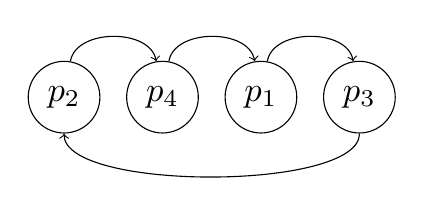
\begin{tikzpicture}[main/.style = {draw, circle}, scale=1.25, transform shape] 
                            \node[main] (1) {$p_2$};
                            \node[main] (2) [right of=1] {$p_4$};
                            \node[main] (3) [right of=2] {$p_1$};
                            \node[main] (4) [right of=3] {$p_3$};
                            \draw[->] (1) to [out=80, in=100, looseness=1] (2);
                            \draw[->] (2) to [out=80, in=100, looseness=1] (3);
                            \draw[->] (3) to [out=80, in=100, looseness=1] (4);
                            \draw[->] (4) to [out=270, in=270, looseness=0.5] (1);
                        \end{tikzpicture} 
                    \end{center}
                    \tcblower
                    Si \texttt{group\_by\_team} renvoie :
                    
                    \texttt{[[($p_1, p_2$), ($p_2, p_3$), ($p_3, p_4$), ($p_4, p_1$)]]}
                    
                    alors un tirage possible est : 
                    
                    \texttt{[($p_2, p_4$), ($p_4, p_1$), ($p_1, p_3$), ($p_3, p_2$)]}
                \end{example}
                \item \bigbreak\underline{Les participants sont répartis dans plusieurs groupes :} La méthode utilisée consiste à fabriquer les couples en parcourant successivement les autres groupes. On donne cet algorithme sous forme de pseudo-code :
                \begin{longlisting}
                    \caption{Pseudo-code algorithme de création des paires}
                    \begin{minted}[linenos]{python}
L <- liste renvoyée par group_by_team 

Mélanger L
L_UPDATED <- copie de L # sera L privée de ceux qui n'ont pas encore de cadeau
R <- [] # liste des paires
Pour chaque GROUPE dans L :
    Pour chaque DONNEUR dans groupe :
        L_PRETENDANTS <- groupe après GROUPE dans L_UPDATED
        RECEVEUR <- Tirer aléatoirement dans L_PRETENDANTS 
        Ajouter (DONNEUR, RECEVEUR) à R
        Retirer RECEVEUR de L_UPDATED
    Fin de Pour
Fin de Pour

Renvoyer R
                    \end{minted}
                \end{longlisting}
                \begin{example}{}{}
                    Prenons \texttt{[[$p_1, p_2, p_3$], [$p_4, p_5, p_6$], [$p_7, p_8, p_9$]]} la liste renvoyée par \texttt{group\_by\_team}.
                    \bigbreak
                    \begin{minipage}[h]{0.48\textwidth}
                        \begin{center}
                            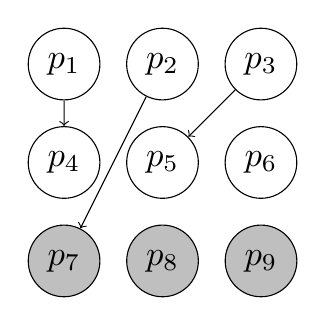
\begin{tikzpicture}[main/.style = {draw, circle}, scale=1.25, transform shape] 
                                \node[main, fill=white] (1) {$p_1$};
                                \node[main, fill=white] (2) [right of=1] {$p_2$};
                                \node[main, fill=white] (3) [right of=2] {$p_3$};
                                \node[main] (4) [below of=1] {$p_4$};
                                \node[main] (5) [below of=2] {$p_5$};
                                \node[main] (6) [below of=3] {$p_6$};
                                \node[main, fill=lightgray] (7) [below of=4] {$p_7$};
                                \node[main, fill=lightgray] (8) [below of=5] {$p_8$};
                                \node[main, fill=lightgray] (9) [below of=6] {$p_9$};
                                \draw[->] (1) to (4);
                                \draw[->] (2) to (7);
                                \draw[->] (3) to (5);
                            \end{tikzpicture} 
                        \end{center}        
                    \end{minipage}
                    \begin{minipage}[h]{0.48\textwidth}
                        \textbf{Étape 1 :} groupe \texttt{[$p_1, p_2, p_3$]}          
                        
                        $p_1 \leadsto $ tirage aléatoire dans \texttt{[$p_4, p_5, p_6$]}
                        
                        $p_2 \leadsto $ tirage aléatoire dans \texttt{[$p_7, p_8, p_9$]}
                        
                        $p_3 \leadsto $ tirage aléatoire dans \texttt{[$p_5, p_6$]}
                    \end{minipage}
                    \bigbreak
                    \begin{minipage}[h]{0.48\textwidth}
                        \begin{center}
                            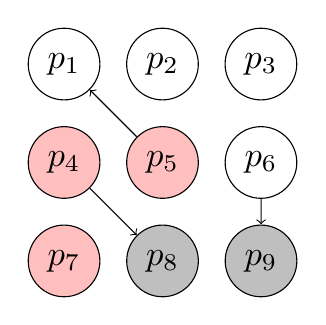
\begin{tikzpicture}[main/.style = {draw, circle}, scale=1.25, transform shape] 
                                \node[main, fill=white] (1) {$p_1$};
                                \node[main, fill=white] (2) [right of=1] {$p_2$};
                                \node[main, fill=white] (3) [right of=2] {$p_3$};
                                \node[main, fill=pink] (4) [below of=1] {$p_4$};
                                \node[main, fill=pink] (5) [below of=2] {$p_5$};
                                \node[main] (6) [below of=3] {$p_6$};
                                \node[main, fill=pink] (7) [below of=4] {$p_7$};
                                \node[main, fill=lightgray] (8) [below of=5] {$p_8$};
                                \node[main, fill=lightgray] (9) [below of=6] {$p_9$};
                                \draw[->] (4) to (8);
                                \draw[->] (5) to (1);
                                \draw[->] (6) to (9);
                            \end{tikzpicture} 
                        \end{center}        
                    \end{minipage}
                    \begin{minipage}[h]{0.48\textwidth}
                        \textbf{Étape 2 :} groupe \texttt{[$p_4, p_5, p_6$]}          
                        
                        $p_4 \leadsto $ tirage aléatoire dans \texttt{[$p_8, p_9$]}
                        
                        $p_5 \leadsto $ tirage aléatoire dans \texttt{[$p_1, p_2, p_3$]}
                        
                        $p_6 \leadsto $ tirage aléatoire dans \texttt{[$p_9$]}
                        
                        \color{pink!150}{participant ayant déjà reçu un cadeau}
                    \end{minipage}
                    \bigbreak
                    \begin{minipage}[h]{0.48\textwidth}
                        \begin{center}
                            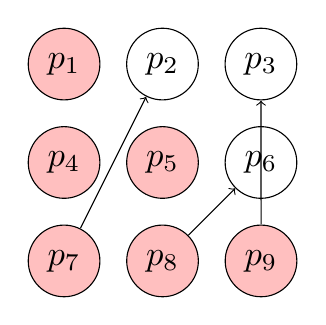
\begin{tikzpicture}[main/.style = {draw, circle}, scale=1.25, transform shape] 
                                \node[main, fill=pink] (1) {$p_1$};
                                \node[main, fill=white] (2) [right of=1] {$p_2$};
                                \node[main, fill=white] (3) [right of=2] {$p_3$};
                                \node[main, fill=pink] (4) [below of=1] {$p_4$};
                                \node[main, fill=pink] (5) [below of=2] {$p_5$};
                                \node[main] (6) [below of=3] {$p_6$};
                                \node[main, fill=pink] (7) [below of=4] {$p_7$};
                                \node[main, fill=pink] (8) [below of=5] {$p_8$};
                                \node[main, fill=pink] (9) [below of=6] {$p_9$};
                                \draw[->] (7) to (2);
                                \draw[->] (8) to (6);
                                \draw[->] (9) to (3);
                            \end{tikzpicture} 
                        \end{center}        
                    \end{minipage}
                    \begin{minipage}[h]{0.48\textwidth}
                        \textbf{Étape 3 :} groupe \texttt{[$p_7, p_8, p_9$]}          
                        
                        $p_7 \leadsto $ tirage aléatoire dans \texttt{[$p_2, p_3$]}
                        
                        $p_8 \leadsto $ tirage aléatoire dans \texttt{[$p_6$]}
                        
                        $p_9 \leadsto $ tirage aléatoire dans \texttt{[$p_3$]}
                    \end{minipage}
                    \bigbreak
                        \texttt{[($p_1, p_4$), ($p_2, p_7$), ($p_3, p_5$), ($p_4, p_8$), ($p_5, p_1$), ($p_6, p_9$), ($p_7, p_2$), ($p_8, p_6$), ($p_9, p_3$)]}.
                \end{example}
            \end{itemize}
    \section{Chiffrement}
        \subsection{Cryptosystème d'\textsc{ElGamal}}
            Une autre contrainte du tirage est la sécurité, il faut pouvoir garantir la confidentialité des données lorsque les informations sont stockées et manipulées afin d'éviter la triche. 
            \begin{definition}{Algorithme de chiffrement homomorphe}{}
                Système possédant des caractéristiques algébriques qui lui permettent de commuter avec certaines opérations mathématiques, c'est-à-dire qu'il permet d'opérer un obscurcissement sur des valeurs numériques tout en conservant les propriétés permettant les dites opérations.\footnotemark
            \end{definition}
            \footnotetext{\url{https://fr.wikipedia.org/wiki/Chiffrement_homomorphe}}
            Le chiffrement homomorphe semble être l'outil adapté pour satisfaire la sécurité tout en étant capable de continuer à manipuler les données. Le cryptosystème retenu et présenté ici est celui d'\textsc{ElGamal}, il fonctionne avec une clé publique qui permet de chiffrer les données et une clé privée qui pour les déchiffrer.
            \bigbreak
            \important{Notations :} on pose \texttt{NBITS} un entier strictement supérieur à 1, $q$ un entier premier de \texttt{NBITS} et $g$ un générateur de $\Z_{/q\Z}$ choisi aléatoirement entre $2$ et $q$.
            \bigbreak 
            Pour générer les deux clés, on prend $x$ un entier quelconque de $\ie{2^{\texttt{NBITS}-1},q-1}$ et avec $h\egdef g^x\text{ mod }q$ les clés sont données par
            \begin{tcolorbox}[hbox, center]
                clé privée : \texttt{sk} $\egdef x$ | clé publique : \texttt{pk} $\egdef (q, g, h)$
            \end{tcolorbox}
            \bigbreak
            Pour chiffrer un entier $m$, on prend $r$ un entier quelconque de $\ie{2^{\texttt{NBITS}-1},q-1}$ et le message chiffré est 
            \begin{tcolorbox}[hbox, center]
                $(c_1, c_2)\egdef (g^r\text{ mod }q, m\times h^r\text{ mod }q)$
            \end{tcolorbox}
            \begin{theorem}{Déchiffrer un message}{dechiffrer}
                Soit $(c_1, c_2)$ un message chiffré.
                
                Le message en clair est $\dfrac{c_2}{c_1^x}\text{ mod }q$.
            \end{theorem}
            \begin{proof}
                (Théorème \ref{th:dechiffrer})
                
                Soit $(c_1, c_2)$ un message chiffré.
                \[\dfrac{c_2}{c_1^x}\text{ mod }q = \dfrac{m\times h^r}{(g^r)^x}\text{ mod }q = \dfrac{m\times (g^x)^r}{(g^r)^x}\text{ mod }q = \dfrac{m\times g^{xr}}{g^{xr}}\text{ mod }q = m\text{ mod }q\]
            \end{proof}
            \begin{theorem}{Homomorphe multiplicatif}{multipl}
                Le cryptosystème d'\textsc{ElGamal} est homomorphe vis-à-vis de la multiplication. C'est-à-dire que si $m_1$ et $m_2$ sont deux entiers chiffrés respectivement par $(c_{1, 1}, c_{1, 2})$ et $(c_{2, 1}, c_{2, 2})$ alors $(c_{1, 1}\times c_{2, 1}, c_{1, 2}\times c_{2, 2})$ est la représentation chiffrée de $m_1\times m_2$.
            \end{theorem}
            \begin{proof}
                (Théorème \ref{th:multipl})
                
                Soit $m_1$ et $m_2$ deux entiers chiffrés respectivement par $(c_{1, 1}, c_{1, 2})$ et $(c_{2, 1}, c_{2, 2})$.
                
                \[\dfrac{c_{1, 2}\times c_{2, 2}}{(c_{1, 1}\times c_{2, 1})^x} = \dfrac{m_1\times h^{r_1}\times m_2 \times h^{r_2}}{(g^{r_1}\times g^{r_2})^x} = \dfrac{m_1m_2\times h^{r_1+r_2}}{(g^{r_1+r_2})^x} = \dfrac{m_1m_2\times(g^x)^{r_1+r_2}}{(g^{r_1+r_2})^x} = m_1m_2\text{ mod }q\]
            \end{proof}
        \subsection{Code source}
            La dernière version de ce code est disponible à l'adresse \url{https://github.com/StanislasMzx/Secret-Santa-TIPE}
            \begin{longlisting}
                \caption{Fichier elgamal.py}
                \begin{minted}[linenos, breaklines, autogobble]{python}
#!/usr/bin/env python3
# -*- coding: utf-8 -*-
"""
Created in 2021

@author: Stanislas MEZUREUX

Copyright (c) 2021 Stanislas MEZUREUX. All rights reserved.
"""

import random

NUMBITS = 1024

# q -> cyclic group order 
# g -> cyclic group generator 
# x -> prvate key
# (q, g, h) where h = g**x mod p -> private key

def gcd(a, b):
    if a < b:
        return gcd(b, a)
    elif a%b == 0:
        return b;
    else:
        return gcd(b, a%b)


# Miller-Rabin
# medium.com/@prudywsh/how-to-generate-big-prime-numbers-miller-rabin-49e6e6af32fb
def is_prime(n, k=128):
    if n == 2 or n == 3:
        return True
    if n <= 1 or n % 2 == 0:
        return False
    s = 0
    r = n - 1
    while r & 1 == 0:
        s += 1
        r //= 2
    for _ in range(k):
        a = random.randrange(2, n - 1)
        x = pow(a, r, n)
        if x != 1 and x != n - 1:
            j = 1
            while j < s and x != n - 1:
                x = pow(x, 2, n)
                if x == 1:
                    return False
                j += 1
            if x != n - 1:
                return False
    return True


def generate_prime_candidate(length):
    p = random.getrandbits(length)
    p |= (1 << length - 1) | 1
    return p


def generate_prime_number(length=1024):
    p = 4
    while not is_prime(p, 128):
        p = generate_prime_candidate(length)
    return p


def keygen():
    q = generate_prime_number(NUMBITS)
    g = random.randint(2, q)
    x = random.randint(2**(NUMBITS-1), q)
    return (x, {'q': q, 'g': g, 'h': pow(g, x, q)})


def encrypt(n, pk):
    q, g, h = pk['q'], pk['g'], pk['h']
    r = random.randint(2**(NUMBITS-1),q)
    return {'c1': pow(g, r, q), 'c2': n*pow(h, r, q)}


def decrypt(n, x, pk):
    return (n['c2']*pow(n['c1'], -x, pk['q']))%pk['q']


def multiply(n1, n2):
    n1c1, n1c2 = n1['c1'], n1['c2']
    n2c1, n2c2 = n2['c1'], n2['c2']
    return {'c1': n1c1*n2c1, 'c2': n1c2*n2c2}
                \end{minted}
            \end{longlisting}
    \section{Preuve à divulgation nulle de connaissance}
            \begin{definition}{Preuve à divulgation nulle de connaissance}{}
                Désigne un protocole sécurisé dans lequel une entité, nommée « fournisseur de preuve », prouve mathématiquement à une autre entité, le « vérificateur », qu'une proposition est vraie sans toutefois révéler d'autres informations que la véracité de la proposition.\footnotemark
            \end{definition}
            \footnotetext{\url{https://fr.wikipedia.org/wiki/Preuve_à_divulgation_nulle_de_connaissance}}
            L'objectif de cette partie est de pouvoir garantir à tous les participant une fois le tirage effectué, sans faire fuiter d'information,  que le tirage est conforme. C'est à dire que chaque personne engagée dans le père Noël secret donne exactement un cadeau et reçoit exactement un cadeau.
        \subsection{Stockage du tirage}
            Pour pouvoir être en mesure d'implanter la preuve à divulgation nulle de connaissance, la liste de couples qui modélise le tirage doit être stockée. Le cryptosystème introduit dans la section précédent permet de générer un fichier qui contient cette liste sous forme chiffrée lors de l'exécution de l'algorithme. 
            \bigbreak
            Le fait de stocker le tirage sous forme chiffrée permet également de pouvoir envoyer l'issue du tirage par e-mail une nouvelle fois. Par exemple en cas d'erreur sur l'e-mail d'un participant ou pour effectuer un nouveau tirage différent du précédent.
        \subsection{Condition de validité du tirage}
            \begin{theorem}{Condition de validité du tirage}{tirage}
                Soit $n$ le nombre de participants.
                
                Si la liste qui représente le tirage est $[(d_1, r_1), \ldots, (d_n, r_n)]$  et si les participants sont représentés par les entiers de $\ie{1, n}$ alors 
                \[\text{le tirage est valide} \iff
                \begin{cases}
                    \displaystyle\prod_{i=1}^nd_i=n ! \\
                    \displaystyle\prod_{i=1}^nr_i=n !
                \end{cases}\]
            \end{theorem}
            \begin{proof}
                (Théorème \ref{th:tirage})
                
                Soit $n$ le nombre de participants.
                
                Soit $[(d_1, r_1), \ldots, (d_n, r_n)]$  la liste qui représente le tirage avec $\forall i\in\ie{1, n}, d_i\in\ie{1, n}$ et $r_i\in\ie{1, n}$.
                \bigbreak
                \fbox{$\Rightarrow$} Si le tirage est valide, chaque participant donne exactement un cadeau et reçoit exactement un cadeau \textit{i.e.}
                $\forall(i, j)\in\ie{1, n}^2,i\neq j\Rightarrow (d_i\neq d_j \text{ et } r_i \neq r_j)$
                
                Comme $\forall i\in\ie{1, n}, d_i\in\ie{1, n}$ et $r_i\in\ie{1, n}, 
                \begin{cases}
                    \displaystyle\prod_{i=1}^nd_i=n ! \\
                    \displaystyle\prod_{i=1}^nr_i=n !
                \end{cases}$
                \bigbreak
                \fbox{$\Leftarrow$} 
                \[\prod_{i=1}^nd_i=n ! \Rightarrow \prod_{i=1}^nd_i=\prod_{i=1}^ni \Rightarrow \forall(i, j)\in\ie{1, n}^2,i\neq j\Rightarrow (d_i\neq d_j \text{ et } r_i \neq r_j)\]
                Cela signifie que le tirage est valide.
            \end{proof}
    \section{Code source}
        La dernière version de ce code est disponible à l'adresse \url{https://github.com/StanislasMzx/Secret-Santa-TIPE}
            \begin{longlisting}
                \caption{Fichier SecretSanta.py}
                \begin{minted}[linenos, breaklines, autogobble]{python}
#!/usr/bin/env python3
# -*- coding: utf-8 -*-
"""
Created in 2021

@author: Stanislas MEZUREUX

Copyright (c) 2021 Stanislas MEZUREUX. All rights reserved.
"""

import smtplib
from random import shuffle
import copy
import secrets
import time
import elgamal as eg
from math import factorial

AMOUNT = 10
NAME = 'MPSI1 227/228'
DATE = '03/01/2022'


class TooMuchInTheTeam(Exception):
    pass


def nb_participants_check(L):
    for i, team in enumerate(L):
        M = [e for A in L[:i]+L[i+1:] for e in A]
        if M != [] and len(M) < len(L[i]):
            raise TooMuchInTheTeam(f"Too much participants in {team[0][3]}")


def csv_to_list(data):
    with open(data) as f:
        L = f.read().splitlines()
    L = L[1:]
    for i, e in enumerate(L):
        L[i] = [i] + e.split(',')
    return L


def group_by_team(L):
    teams = []
    for e in L:
        if e[3] not in teams:
            teams.append(e[3])
    nb_teams = len(teams)
    M = [[] for _ in range(nb_teams)]
    for i, team in enumerate(teams):
        for e in L:
            if e[3] == team:
                M[i].append(e[0])
    return M


def make_pairs(L, pk):
    nb_teams = len(L)
    if nb_teams == 1:
        M = L[0].copy()
        shuffle(M)
        length = len(M)
        R = [(0, 0)]*length
        for i in range(length):
            R[i] = (eg.encrypt(M[i]+1, pk),
                    eg.encrypt(M[(i+1) % length]+1, pk))
        with open('secret_santa_draw.py', 'w') as f:
            f.write(f'draw = {R}')
        return R
    R = []
    M = copy.deepcopy(L)
    shuffle(M)
    L_new = copy.deepcopy(M)
    for i, team in enumerate(L_new):
        for j, e in enumerate(L_new[i]):
            if len(M) == 1:
                M_next = M[0]
            else:
                M_next = (M[:i]+M[i+1:])[(j+1) % (len(M)-1)]
            M_next_len = len(M_next)
            k = secrets.randbelow(M_next_len)
            gift_to = M_next[k]
            R.append((eg.encrypt(e+1, pk),
                      eg.encrypt(gift_to+1, pk)))
            with open('example/secret_santa_draw.py', 'w') as f:
                f.write(f'draw = {R}\ndraw_len = {len(R)}')
            del M_next[k]
            if M_next_len == 1:
                M = [e for e in M if e != []]
    return R


def send_email(L, data, sk, pk, display_team=True):
    from_addr = 'secret.santa.tipe@gmail.com'

    server = smtplib.SMTP_SSL('smtp.gmail.com', 465)
    server.set_debuglevel(1)
    server.ehlo

    server.login('secret.santa.tipe@gmail.com', 'password')

    for e_encrypted in L:
        e = (eg.decrypt(e_encrypted[0], sk, pk)-1,
             eg.decrypt(e_encrypted[1], sk, pk)-1)
        to_addrs = data[e[0]][4]
        subject = f"Secret Santa - {NAME}"
        text = (
            f'Bonjour {data[e[0]][1]},\nCette année, tu es en charge du '
            f'cadeau de {data[e[1]][1]} {data[e[1]][2]} '
            f'{"("+data[e[1]][3]+")" if display_team else ""}. Je te rappelle '
            f'que le budget est de {AMOUNT}€ et que la célébration aura lieu '
            f'le {DATE}.\nJoyeux Noël à toi !'
        )

        message = f"Subject: {subject}\nFrom: {from_addr}\nTo: {to_addrs}\n\n"
        message = message + text
        server.sendmail(from_addr, to_addrs, message.encode("utf8"))

        time.sleep(0.1)

    server.quit()


def zero_knowledge_proof(sk, pk):
    import example.secret_santa_draw as ssd
    if ssd.draw_len == 1:
        return True
    gift_from = ssd.draw[0][0]
    gift_to =  ssd.draw[0][1]
    for i in range(1, ssd.draw_len):
        gift_from = eg.multiply(gift_from, ssd.draw[i][0])
        gift_to = eg.multiply(gift_to, ssd.draw[i][1])
    fact = factorial(ssd.draw_len)
    return eg.decrypt(gift_from, sk, pk) == fact and eg.decrypt(gift_to, sk, pk) == fact


def Secret_Santa(data):
    try:
        sk, pk = eg.keygen()
        info = csv_to_list(data)
        L = group_by_team(info)
        nb_teams = len(L)
        nb_participants_check(L)
        R = make_pairs(L, pk)
        print(f'secret key : {sk}')
        print(f'public key : {pk}')
        send_email(R, info, sk, pk, nb_teams != 1)
    except TooMuchInTheTeam as TeamError:
        print(TeamError)


def resend(sk, pk, data):
    try:
        import example.secret_santa_draw as ssd
        info = csv_to_list(data)
        nb_teams = len(ssd.draw)
        send_email(ssd.draw, info, sk, pk, nb_teams != 1)
    except ModuleNotFoundError as Error:
        print(Error)

# Secret_Santa('example/data.csv')
                \end{minted}
            \end{longlisting}
            
\chapter{Combinatoire}
    \section{Cas d'un seul groupe}
        \noindent Ce cas est le même que celui où les $n$ participants sont dans $n$ groupes différents, $n\geqslant 2$. On pose alors
        \begin{itemize}
            \item $A$ : ensemble de $n$ personnes 
            \item $N$ : nombre de permutations sans point fixe (\textit{i.e.} nombre de tirages possibles)
            \item $\overline{N}$: nombre de permutations avec point fixe
            \item $A_i$ : ensemble des permutations à n éléments avec i comme point fixe 
        \end{itemize}
        \begin{theorem}{Cardinal de l'ensemble des tirages possibles pour n groupes}{ref1}
            \[N=n !\left(1+\sum_{k=1}^{n}\dfrac{(-1)^{k+1}}{k !}\right)\]
        \end{theorem}
        \begin{proof}
            (Théorème \ref{th:ref1})
            \begin{align*}
                \overline{N}
                &= \Card\left(\bigcup_{i=1}^{n}A_i\right) & (1) \\
                &= \sum_{k=1}^{n}\left((-1)^{k+1}\sum_{\substack{I\subset\ie{1, n}\\\Card(I)=k}} \Card\left(\bigcap_{i\in{I}}A_i\right)\right) & (2) \\
                &= \sum_{k=1}^{n}\left((-1)^{k+1}\sum_{I\subset\ie{1, n}} (n-k)!\right) & (3) \\
                &= \sum_{k=1}^{n}(-1)^{k+1}{\binom{k}{n}}(n-k)! & (4) \\
                &= \sum_{k=1}^{n}(-1)^{k+1}\dfrac{n !}{k !} 
            \end{align*}
            \textbf{Explications :}
            \begin{itemize}
                \item $(1)\Rightarrow(2)$ : formule du crible de Poincaré 
                \item $(2)\Rightarrow(3)$ : $k$ éléments sont fixés, il y a $(n-k)!$ possibilités de placer les $n-k$ derniers
                \item $(3)\Rightarrow(4)$ : il y a ${\displaystyle\binom{k}{n}}$ parties de $k$ éléments dans $I$ 
            \end{itemize}
            \begin{align*}
                N
                &= n !-\overline{N} \\
                &= n ! - \sum_{k=1}^{n}(-1)^{k+1}\dfrac{n !}{k !} \\
                &= n ! \left(1+\sum_{k=1}^{n}\dfrac{(-1)^{k+1}}{k !}\right)
            \end{align*}
        \end{proof}
    \section{Cas de 2 groupes}
        \noindent Cas de $2p$ participants et $2$ groupes avec $p$ personnes par groupe, $p \geqslant 1$. On pose
        \begin{itemize}
            \item $G_1$ : premier groupe avec $\Card(G_1)= p$
            \item $G_2$ : deuxième groupe avec $\Card(G_2)= p$
            \item $N$ : nombre de tirages possibles
        \end{itemize}
        \begin{theorem}{Cardinal de l'ensemble des tirages possibles pour 2 groupes}{ref2}
            \[N=(p!)^{2}\]
        \end{theorem}
        \begin{proof}
            (Théorème \ref{th:ref2})
            \bigbreak
            On pose : 
            \bigbreak
        \begin{itemize}
            \item $\App{f}{G_1}{G_2}{x}{y}$ : bijective
            \item $\App{g}{G_2}{G_1}{x}{y}$ : bijective
            \item $F$ : ensemble des bijections de $G_1$ dans $G_2$
            \item $G$ : ensemble des bijections de $G_2$ dans $G_1$
        \end{itemize}
        \begin{align*}
            N
            &=\Card(\{(f,g) ; f \in F \text{ et  }g \in G\}) \\
            &=\Card(F\times G) \\
            &=\Card(F)\times \Card(G) \\
            &=(p!)^{2} 
        \end{align*}
        \end{proof}

\addcontentsline{toc}{chapter}{Bibliographie}
\begin{thebibliography}{6}
    \bibitem{bib:1} \textsc{Sjouke Mauw, Sasa Radomirovic, Peter Ryan} : Security protocols for Secret Santa : \textit{Cambridge International Workshop on Security Protocols (2014)}
    \bibitem{bib:2} \textsc{Evgeniy Prikhodko} : Théorie des graphes : \textit{\url{https://binary-machinery.github.io/2021/02/03/secret-santa-graph.html}}
    \bibitem{bib:3} \textsc{Cécile GONÇALVES} : Cryptographie Avancée : \textit{dentification Zéro-Knowledge, Cryptographie distribuée et Chiffrement homomorphe (2015)}
    \bibitem{bib:4} \textsc{Wikipédia} : Cryptosystème d’\textsc{ElGamal} : \textit{\url{https://fr.wikipedia.org/wiki/Cryptosystème_de_ElGamal}}
    \bibitem{bib:5} \textsc{Marc SAGE} : Combinatoire : \textit{7-9 (2008)}
    \bibitem{bib:6} \textsc{Fatima A. Akinola} : On Hamilton cycle decompositions of complete multipartite graphs which are both cyclic and symmetric : \textit{(2021)}
\end{thebibliography}
            
\end{document}
